\section{Performance}
\label{sec:Performance}

  A high statistics Monte Carlo simulation was performed in order to estimate the reconstruction efficiency and resolution of the implemented track-finding and track-fitting algorithms. It was necessarily Monte Carlo based in order to compare the reconstructed events to the simulated truth, thereby highlighting any inefficiencies and inaccuracies within the algorithms, without any additional noise or biases.

  The fitted transverse positions, $(x,y)$, and momenta, $(p_x, p_y, p_z)$, were compared against the the Monte Carlo truth on an event-by-event basis. The reconstructed events were not subject to any cuts or additional requirements over those of real data reconstruction. The Monte Carlo truth data was determined from the simulated track information which was stored at every tracker plane to permit a direct comparison to the reconstructed data. All data sets were compared at the tracker reference surface, the designated measurement location with the MICE cooling channel.

  \subsection{Track Finding Efficiency}
  \label{sec:performance:track_finding}
  For every simulated event, the number of expected tracks was calculated from the Monte Carlo truth. If the simulated track crossed enough tracker planes to create a sufficient number of spacepoints (3 for straight tracks and 4 for helical tracks), a reconstructed track was expected. The reconstructed tracks were then compared for each tracker and compared to the expected track parameters. The efficiency of track finding as a function of the true longtudinal momentum is shown in figure~\ref{fig:track_efficiency_pz}, and similarly as a function of the true transverse momentum in figure~\ref{fig:track_efficiency_pt}.

  \begin{figure}[p]
    \begin{center}
%      \includegraphics[width=0.49\textwidth, angle=0]{08-Performance/upstream_efficiency_pz.pdf}
%      \includegraphics[width=0.49\textwidth, angle=0]{08-Performance/downstream_efficiency_pz.pdf}
      \caption{\label{fig:track_efficiency_pz} The efficiency of reconstructing tracks in the upstream (left) and downstream (right) trackers as a function of the simulated longitudinal momentum.}
    \end{center}
  \end{figure}

  \begin{figure}[p]
    \begin{center}
%      \includegraphics[width=0.49\textwidth, angle=0]{08-Performance/upstream_efficiency_pt.pdf}
%      \includegraphics[width=0.49\textwidth, angle=0]{08-Performance/downstream_efficiency_pt.pdf}
      \caption{\label{fig:track_efficiency_pt} The efficiency of reconstructing tracks in the upstream (left) and downstream (right) trackers as a function of the simulated transverse momentum.}
    \end{center}
  \end{figure}

  Once the 


  \subsection{Reconstruction Resolution}
  \label{sec:performance:resolutions}
  
  Position residuals are shown in figures~\ref{fig:XResidKalman} and \ref{fig:YResidKalman}, and the momentum residuals in figures~\ref{fig:PtResidKalman} to \ref{fig:PzResidKalman}.  The position reconstruction can be seen to agree with the Monte Carlo truth to high precision in both the upstream and downstream trackers. The offset is negligible and the spread is slightly below the tracker fibre thickness, showing that the system is performing at close to optimal.
  
  The transverse momentum similarly shows an excellent agreement with Monte Carlo truth. The residual histograms contain only a very small offset and the spread is $\sim$1~MeV/c in the upstream tracker, and $\sim$1.2~MeV/c in the downstream tracker for the trasverse momentum.  The longitudinal momentum, an intrinsically more difficult measurement for the tracker, still retains an acceptable spread of 4.1~MeV/c in the upstream tracker, and 3.8~MeV/c in the downstream tracker.  There is however a systematic offset present in the distributions, 2~MeV/c in the upstream tracker, and 3.3~MeV/c in the downstream, and the distributions have more pronounced tails than in the transverse cases.  These offsets require further investigation.
  
  Trends in transverse and longitudinal momentum resolution as a function of transverse momentum are shown in figures~\ref{fig:PtPtResolKalman} and \ref{fig:PtPzResolKalman}. A clear increase in resolution can be seen with increasing transverse momentum in all cases, in keeping with expectations.

  \begin{figure}[p]
    \begin{center}
      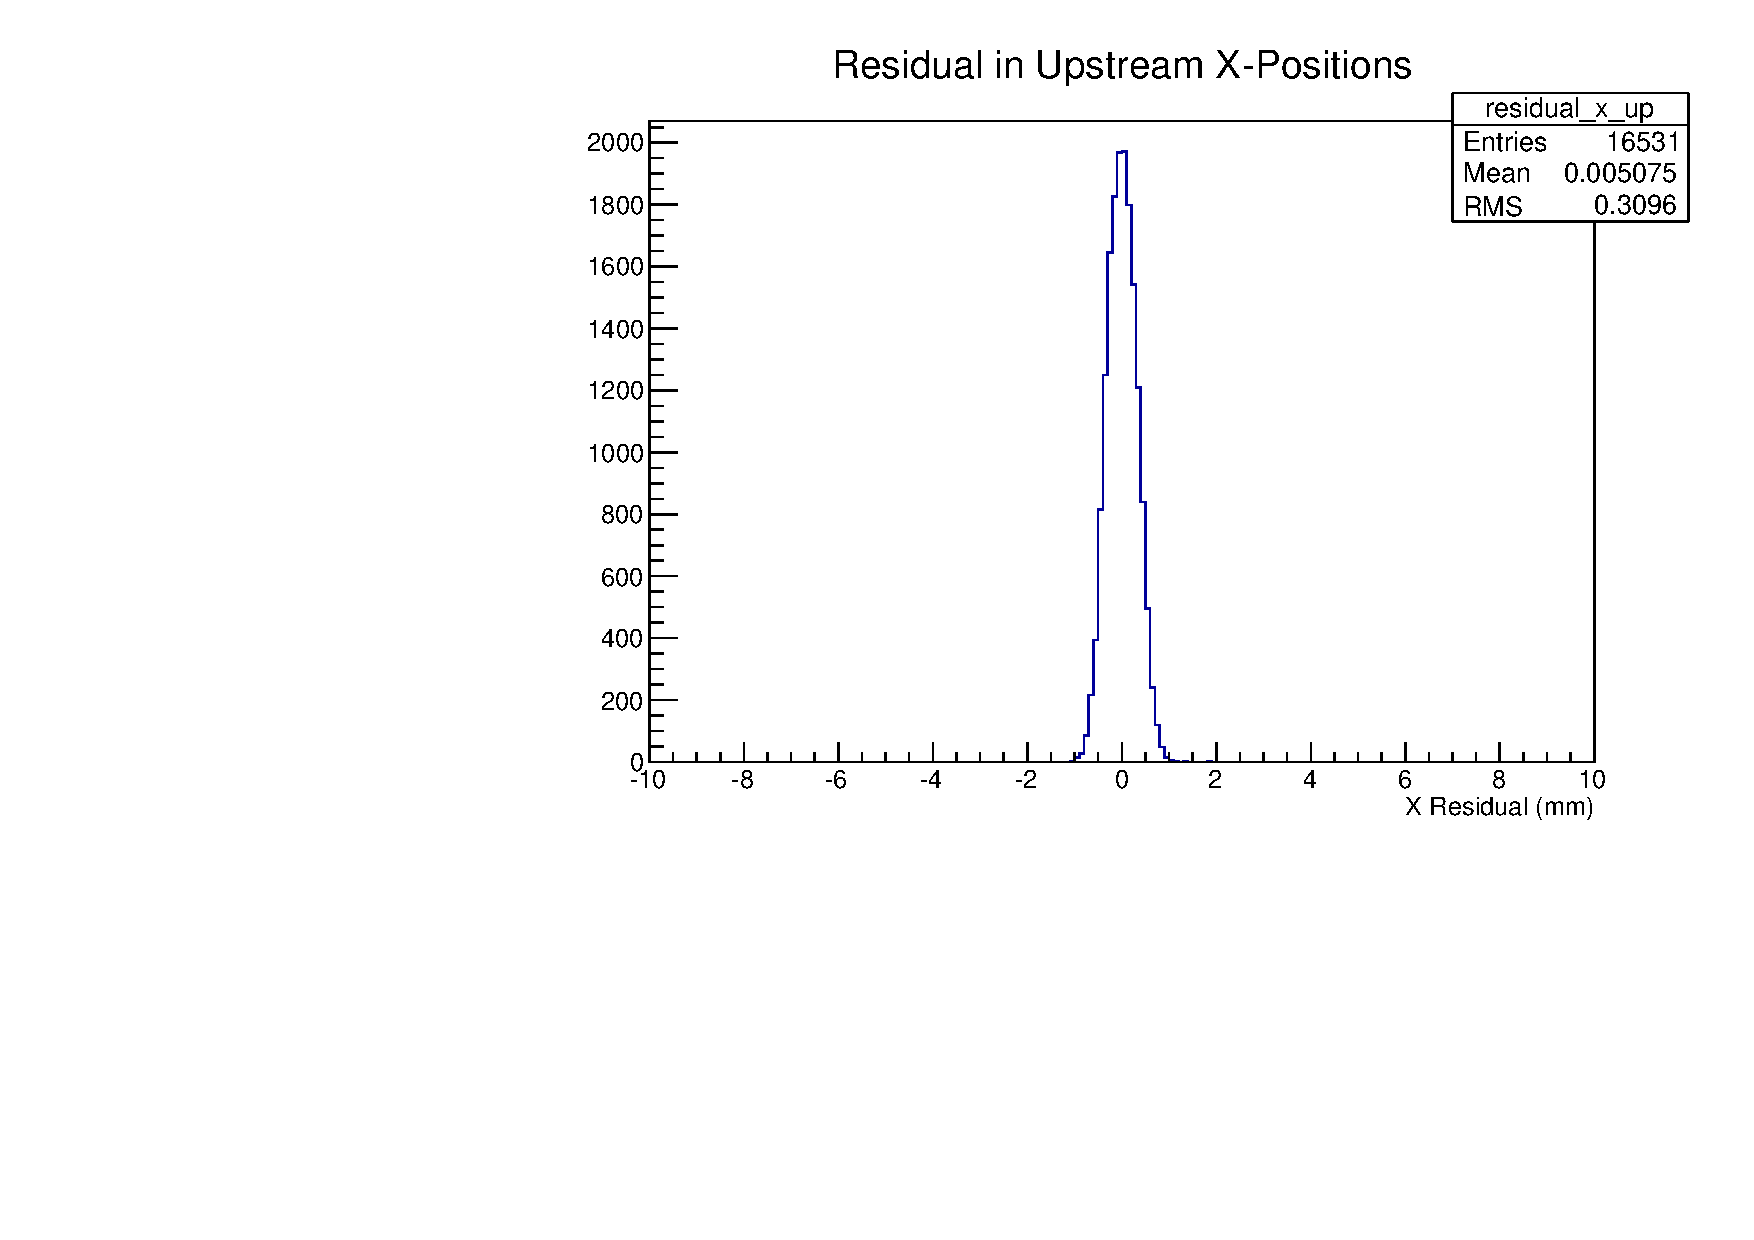
\includegraphics[width=0.49\textwidth, angle=0]{08-Performance/residual_x_up.pdf}
      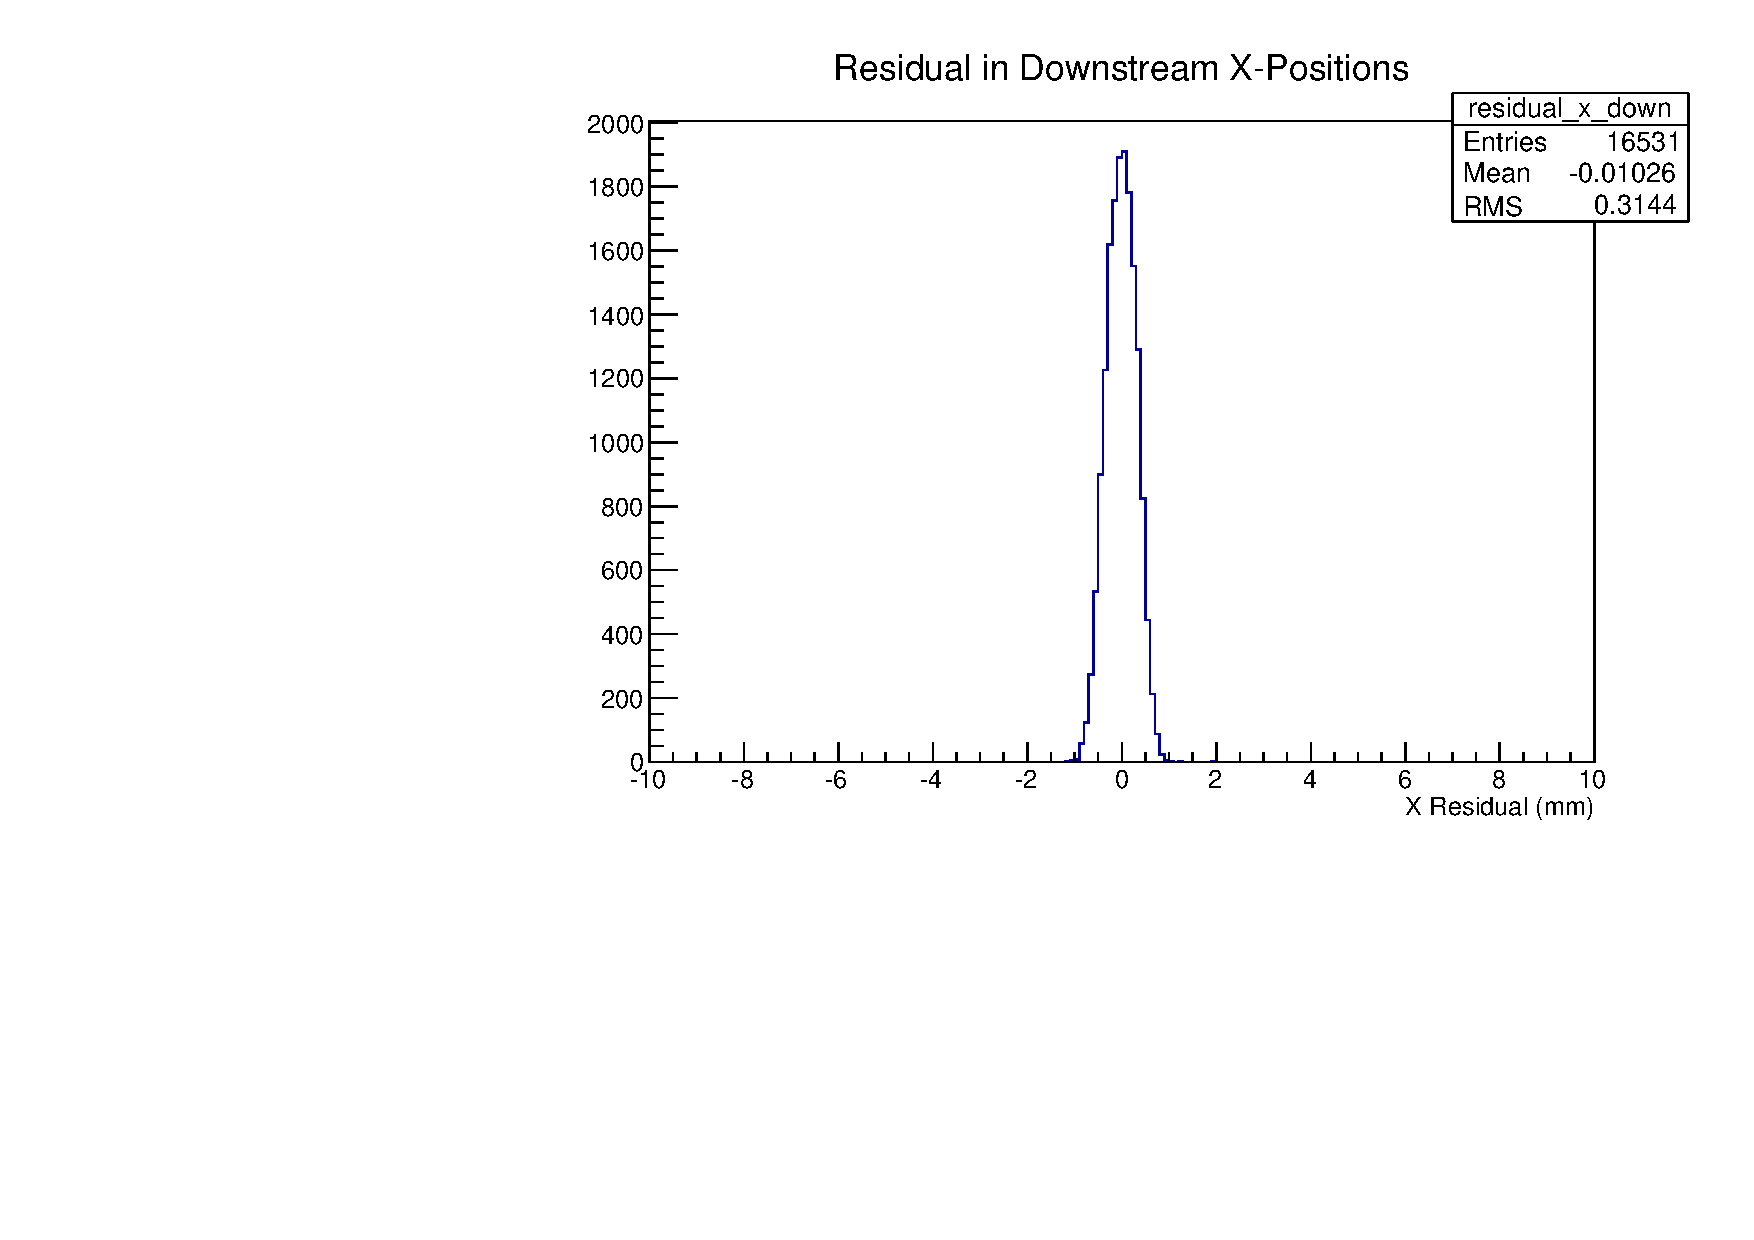
\includegraphics[width=0.49\textwidth, angle=0]{08-Performance/residual_x_down.pdf}
      \caption{\label{fig:XResidKalman} The $x$ residuals of the upstream (left) and downstream (right) trackers for a 6~mm 4D emittance, and 200~MeV/c momentum beam.}
    \end{center}
  \end{figure}
  
    \begin{figure}[p]
    \begin{center}
      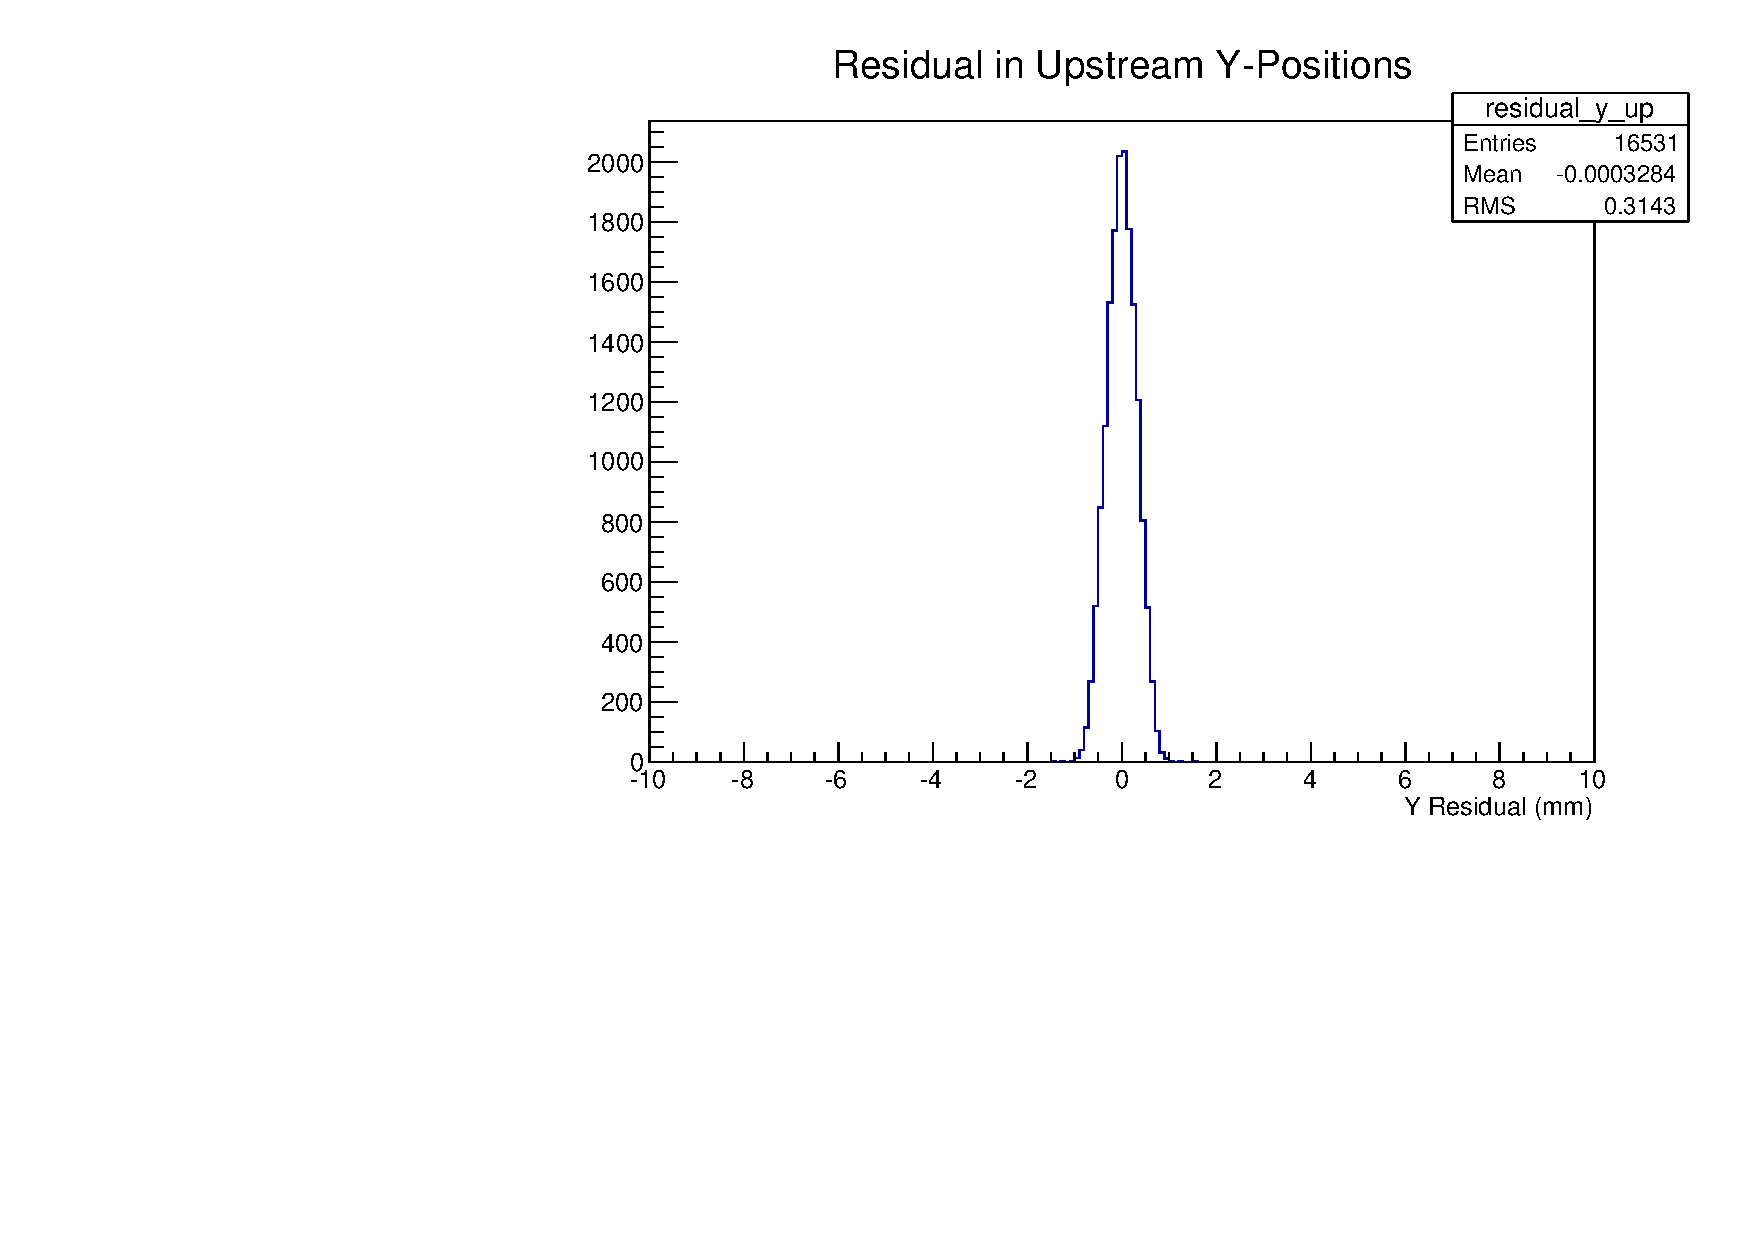
\includegraphics[width=0.49\textwidth, angle=0]{08-Performance/residual_y_up.pdf}
      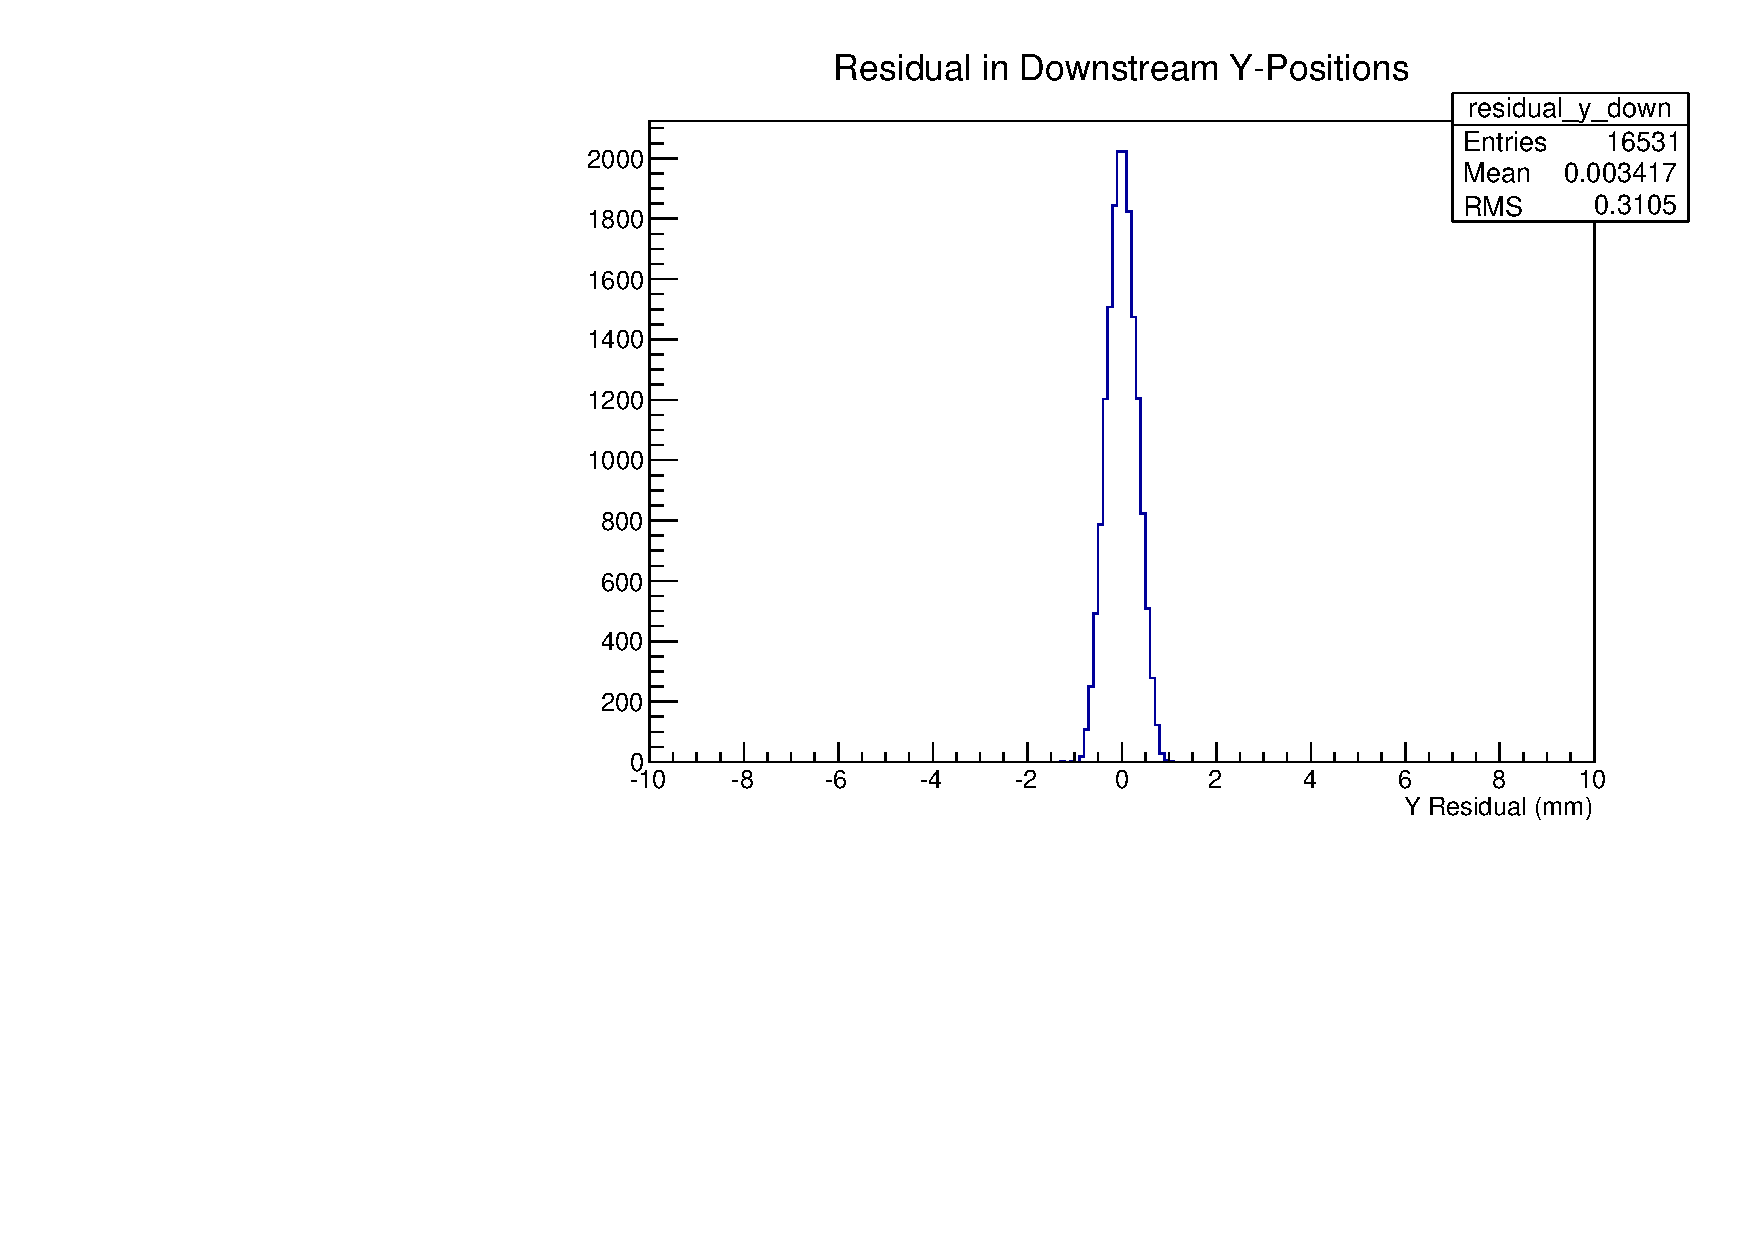
\includegraphics[width=0.49\textwidth, angle=0]{08-Performance/residual_y_down.pdf}
      \caption{\label{fig:YResidKalman} The $y$ residuals of the upstream (left) and downstream (right) trackers for a 6~mm 4D emittance, and 200~MeV/c momentum beam.}
    \end{center}
  \end{figure}
  
  
  \begin{figure}[p]
    \begin{center}
      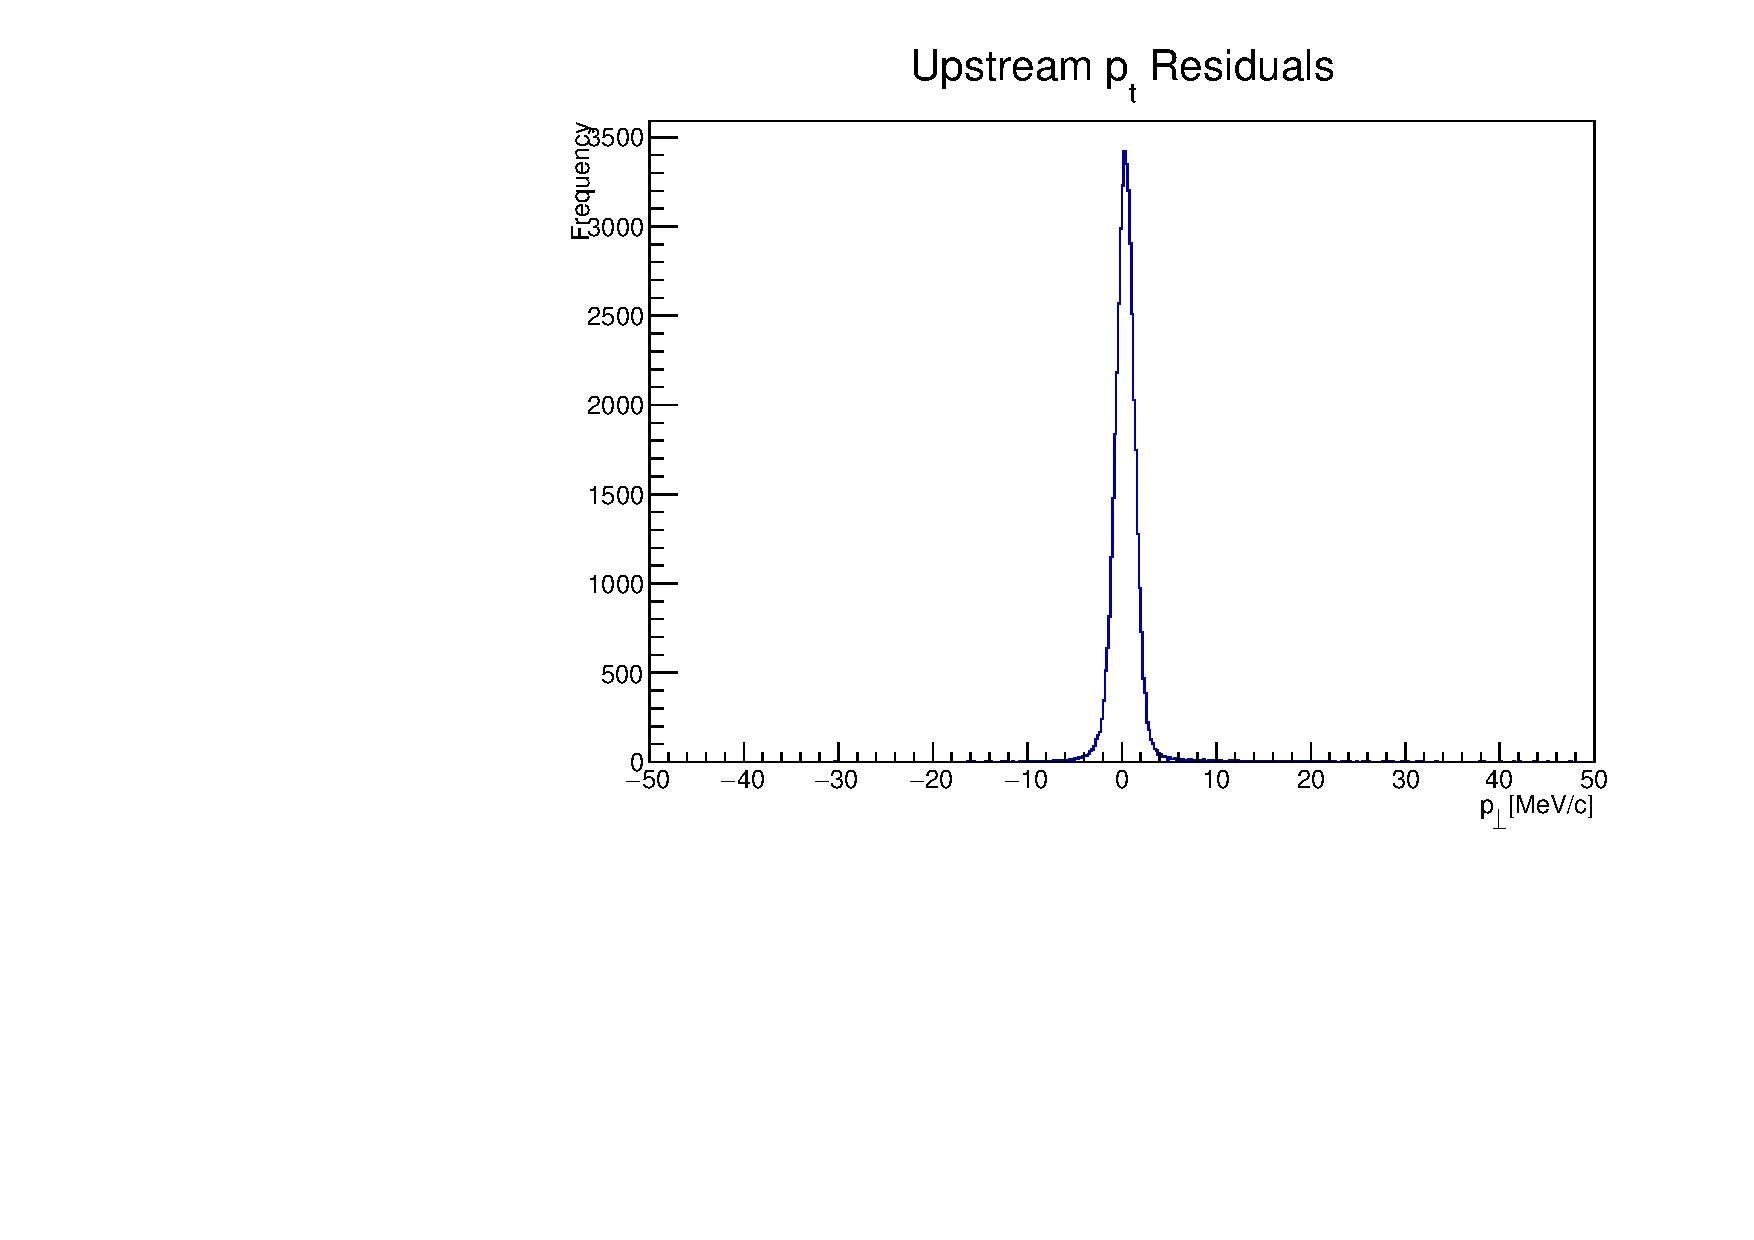
\includegraphics[width=0.49\textwidth, angle=0]{08-Performance/upstream_residual_pt.pdf}
      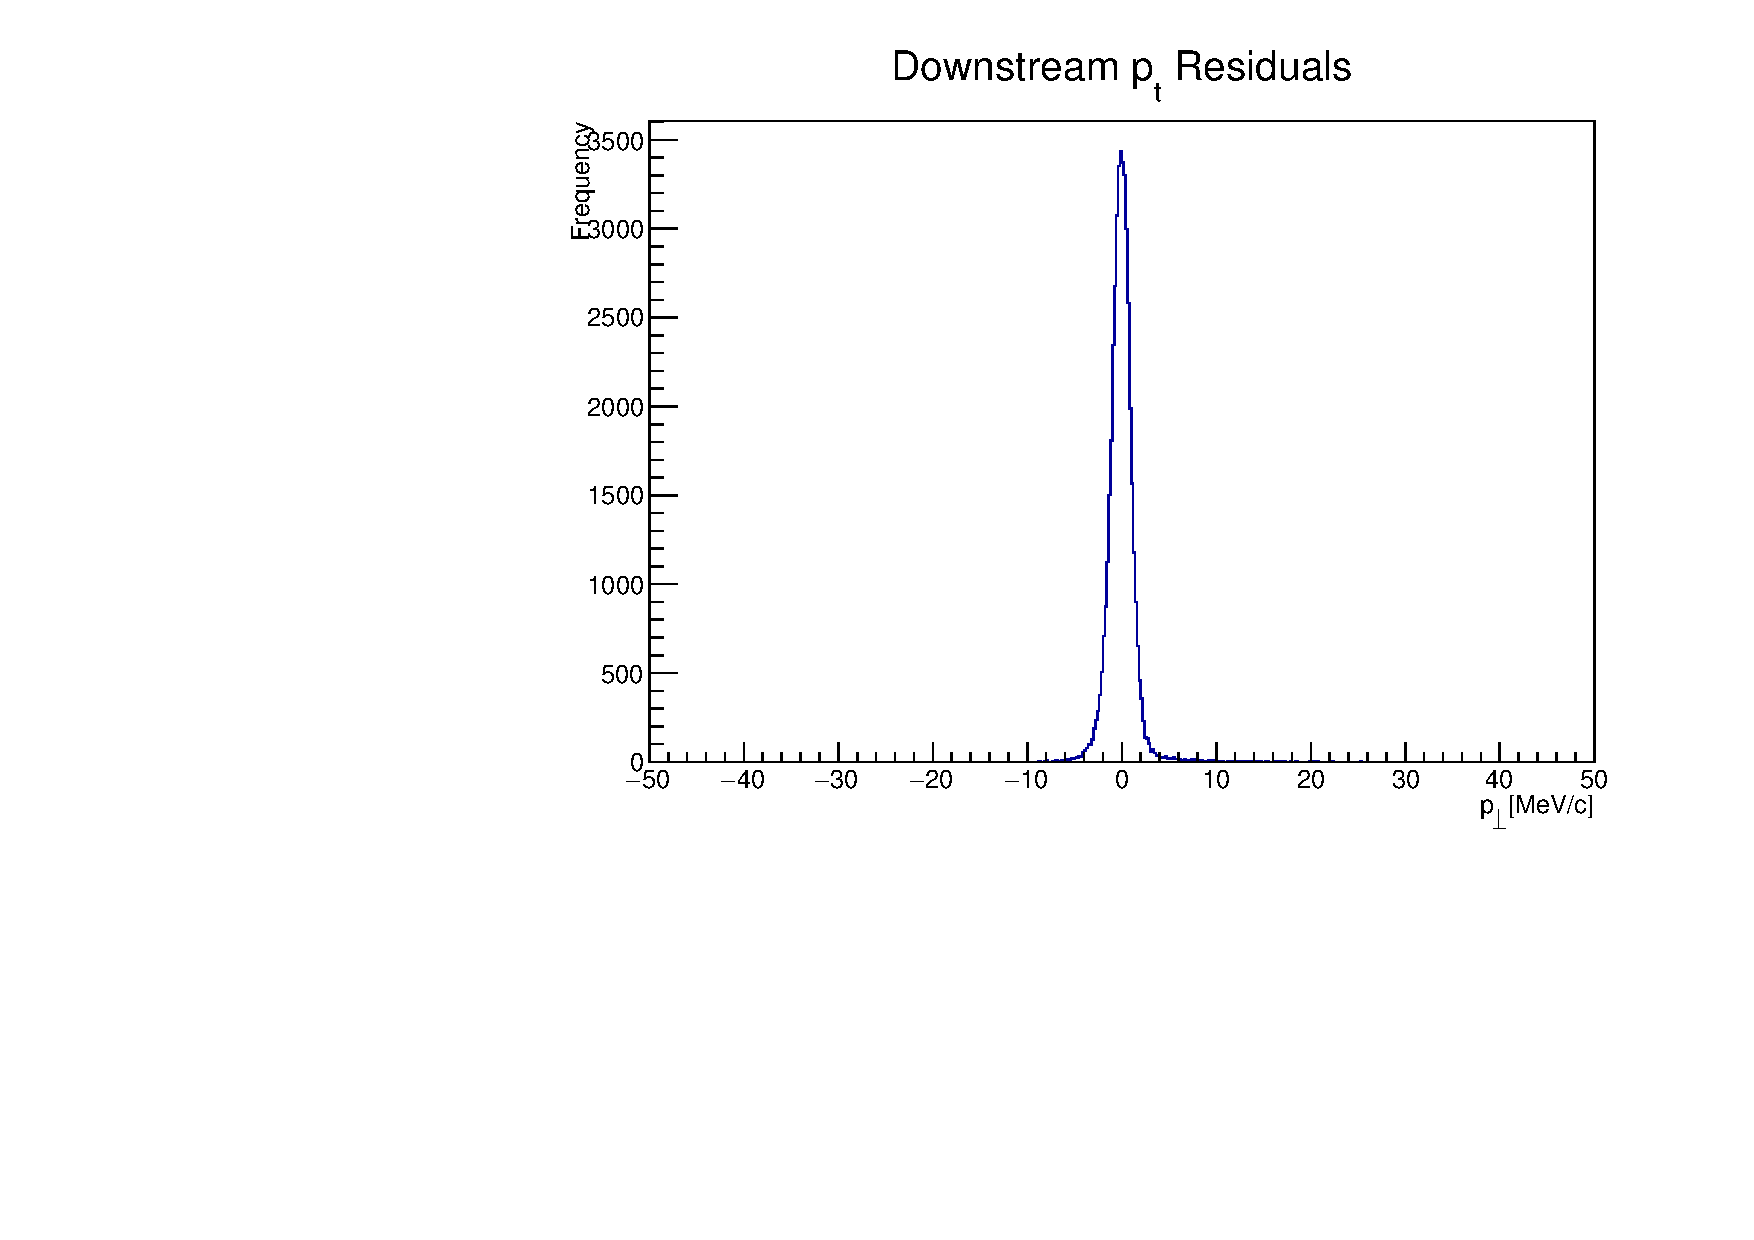
\includegraphics[width=0.49\textwidth, angle=0]{08-Performance/downstream_residual_pt.pdf}
      \caption{\label{fig:PtResidKalman} The $p_t$ residuals of the upstream (left) and downstream (right).}
    \end{center}
  \end{figure}
  
   \begin{figure}[p]
    \begin{center}
      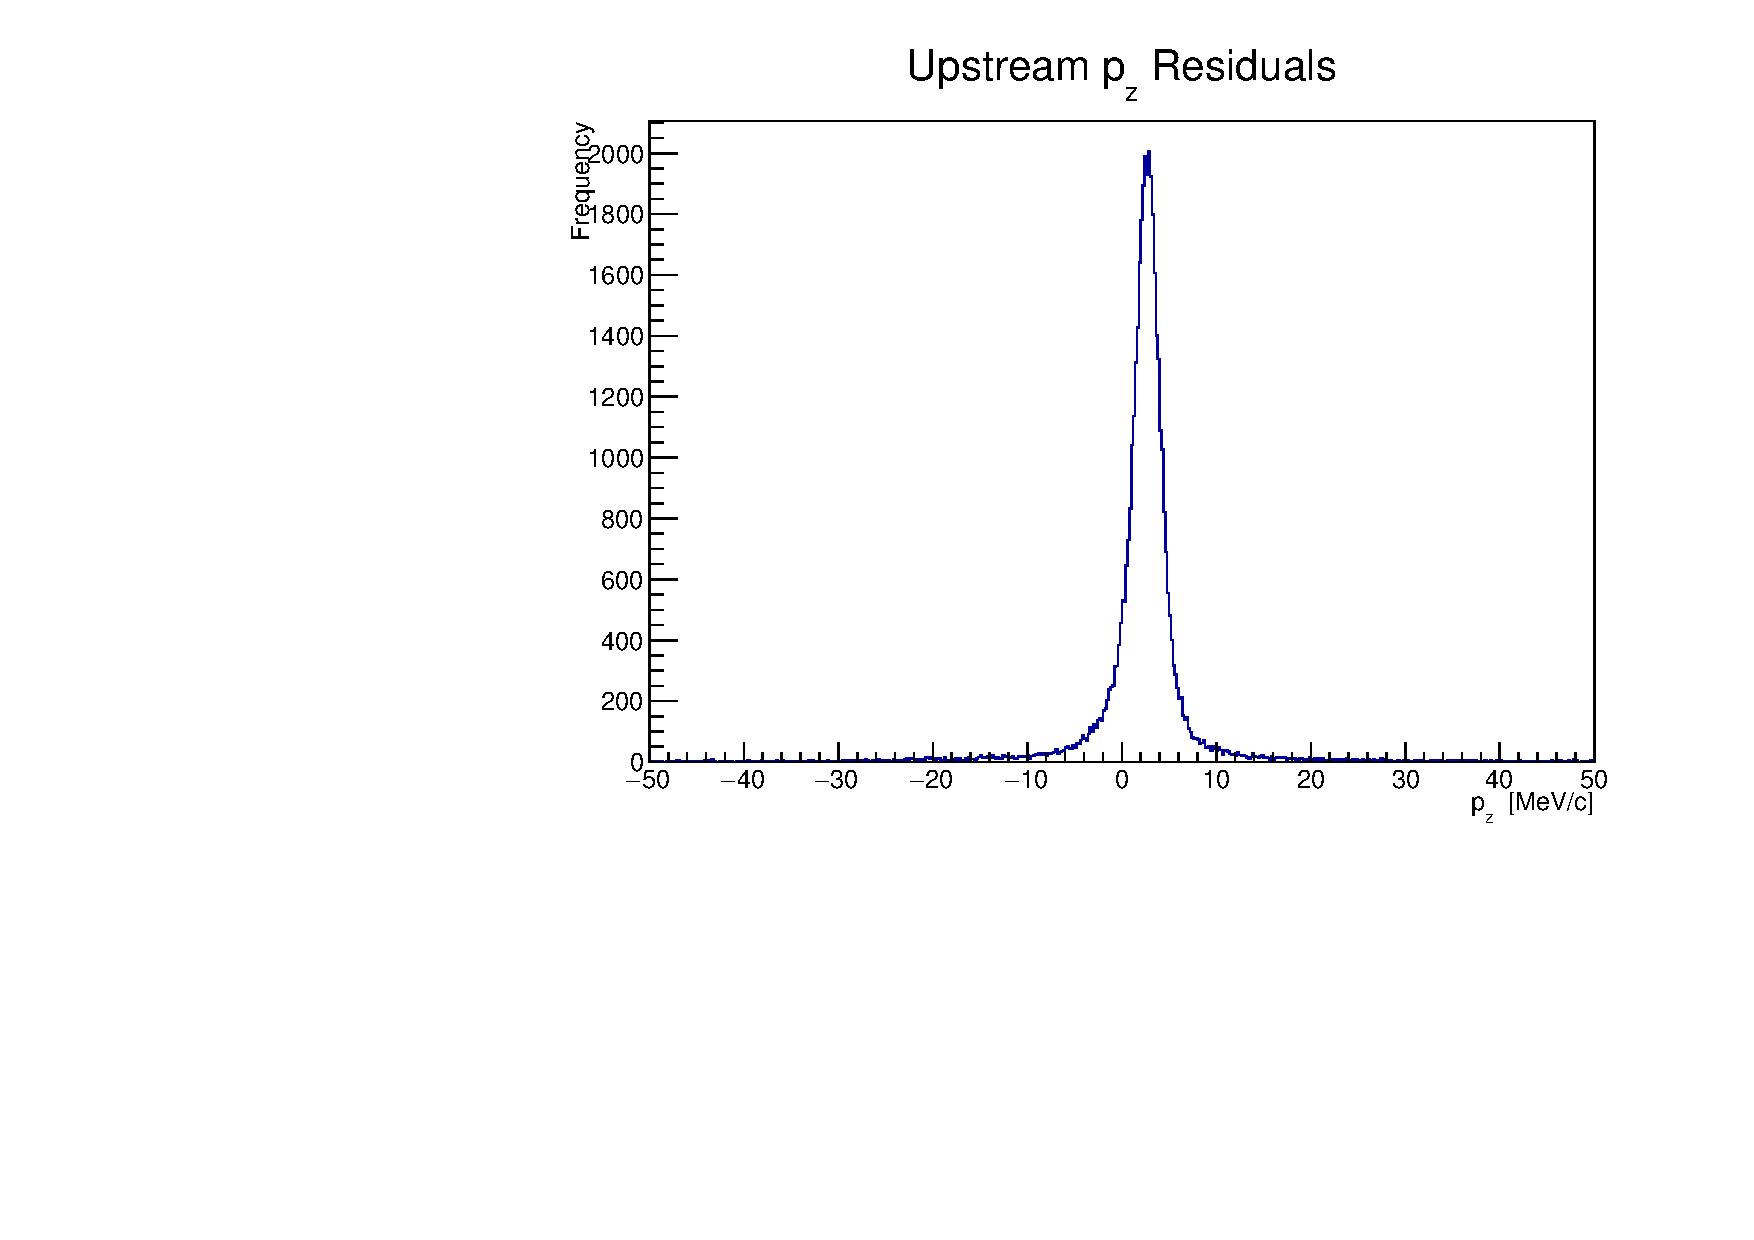
\includegraphics[width=0.49\textwidth, angle=0]{08-Performance/upstream_residual_pz.pdf}
      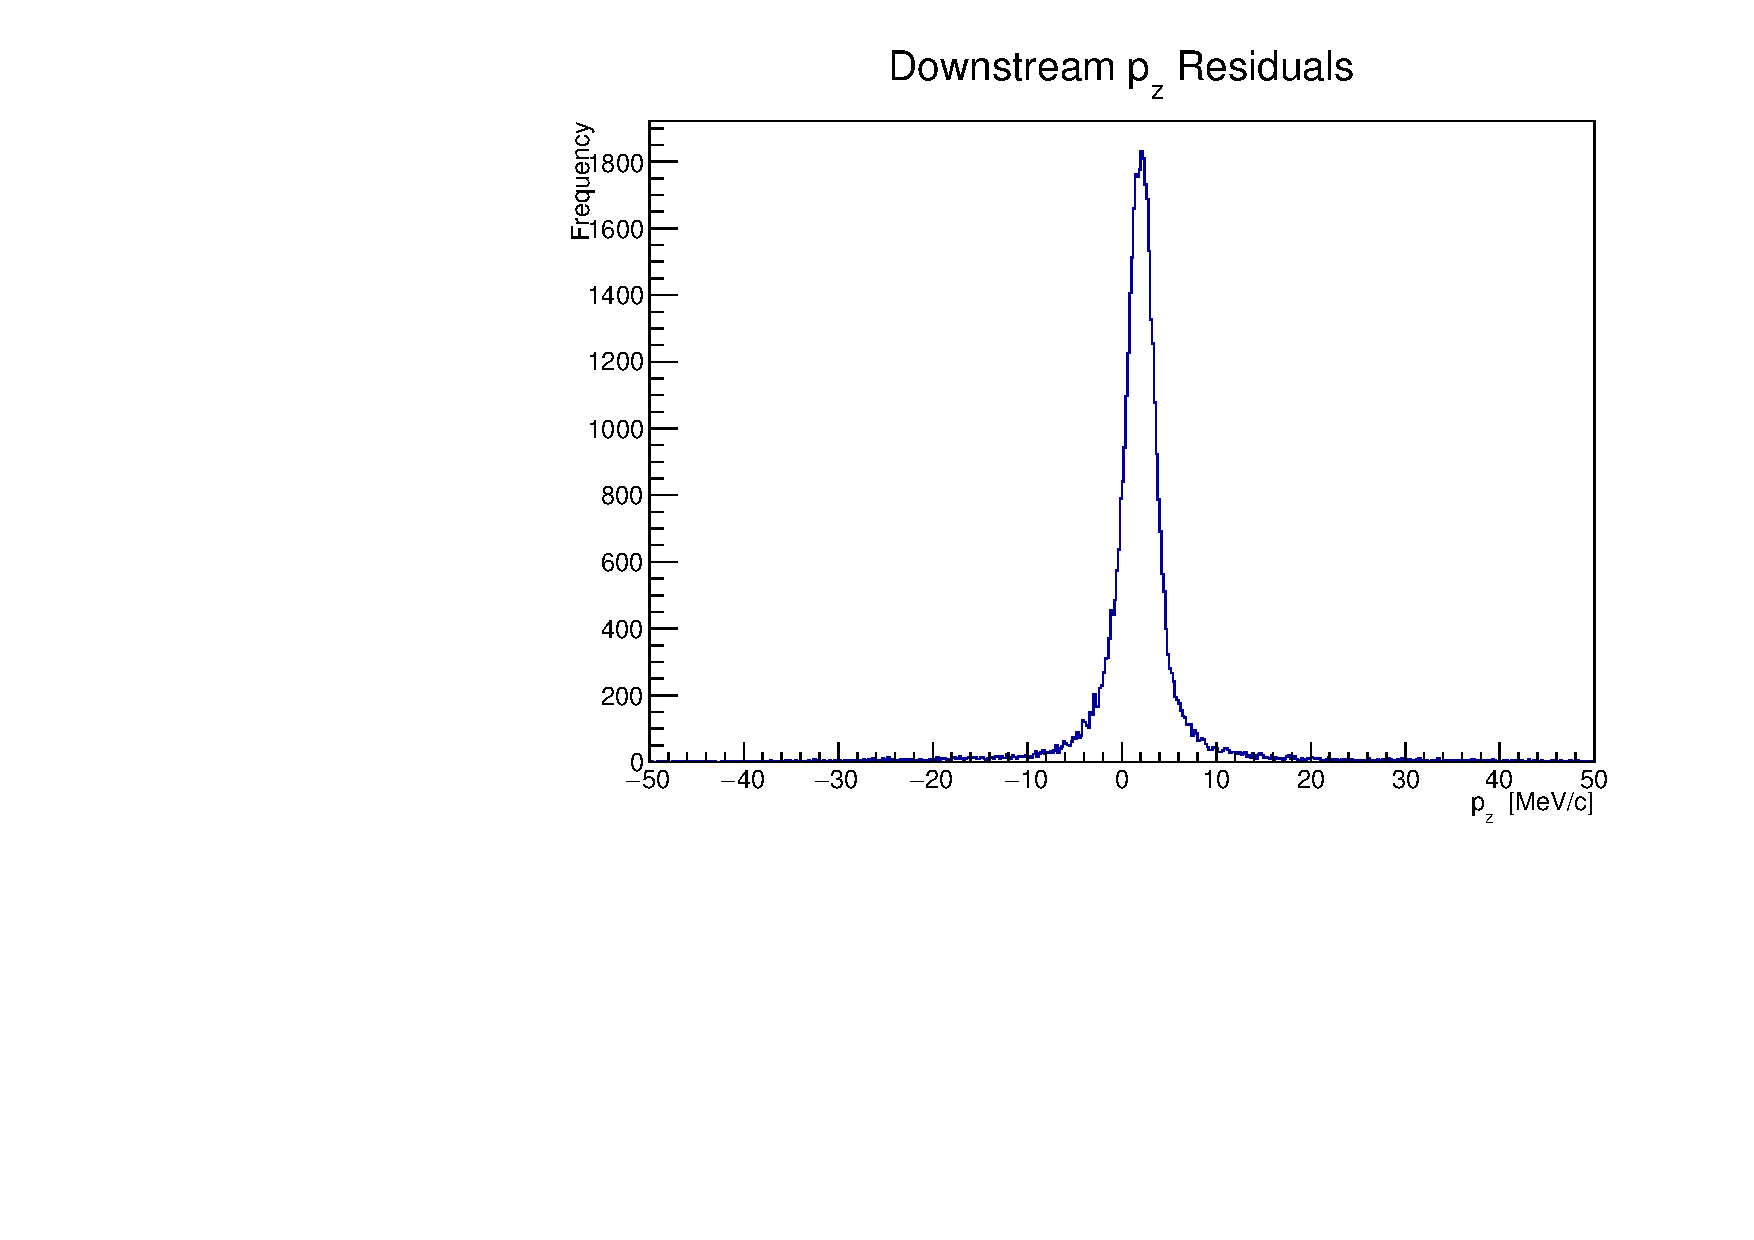
\includegraphics[width=0.49\textwidth, angle=0]{08-Performance/downstream_residual_pz.pdf}
      \caption{\label{fig:PzResidKalman} The $p_z$ residuals of the upstream (left) and downstream (right) trackers for a 6~mm 4D emittance, and 200~MeV/c momentum beam.}
    \end{center}
  \end{figure}
  
  \begin{figure}[p]
   \begin{center}
     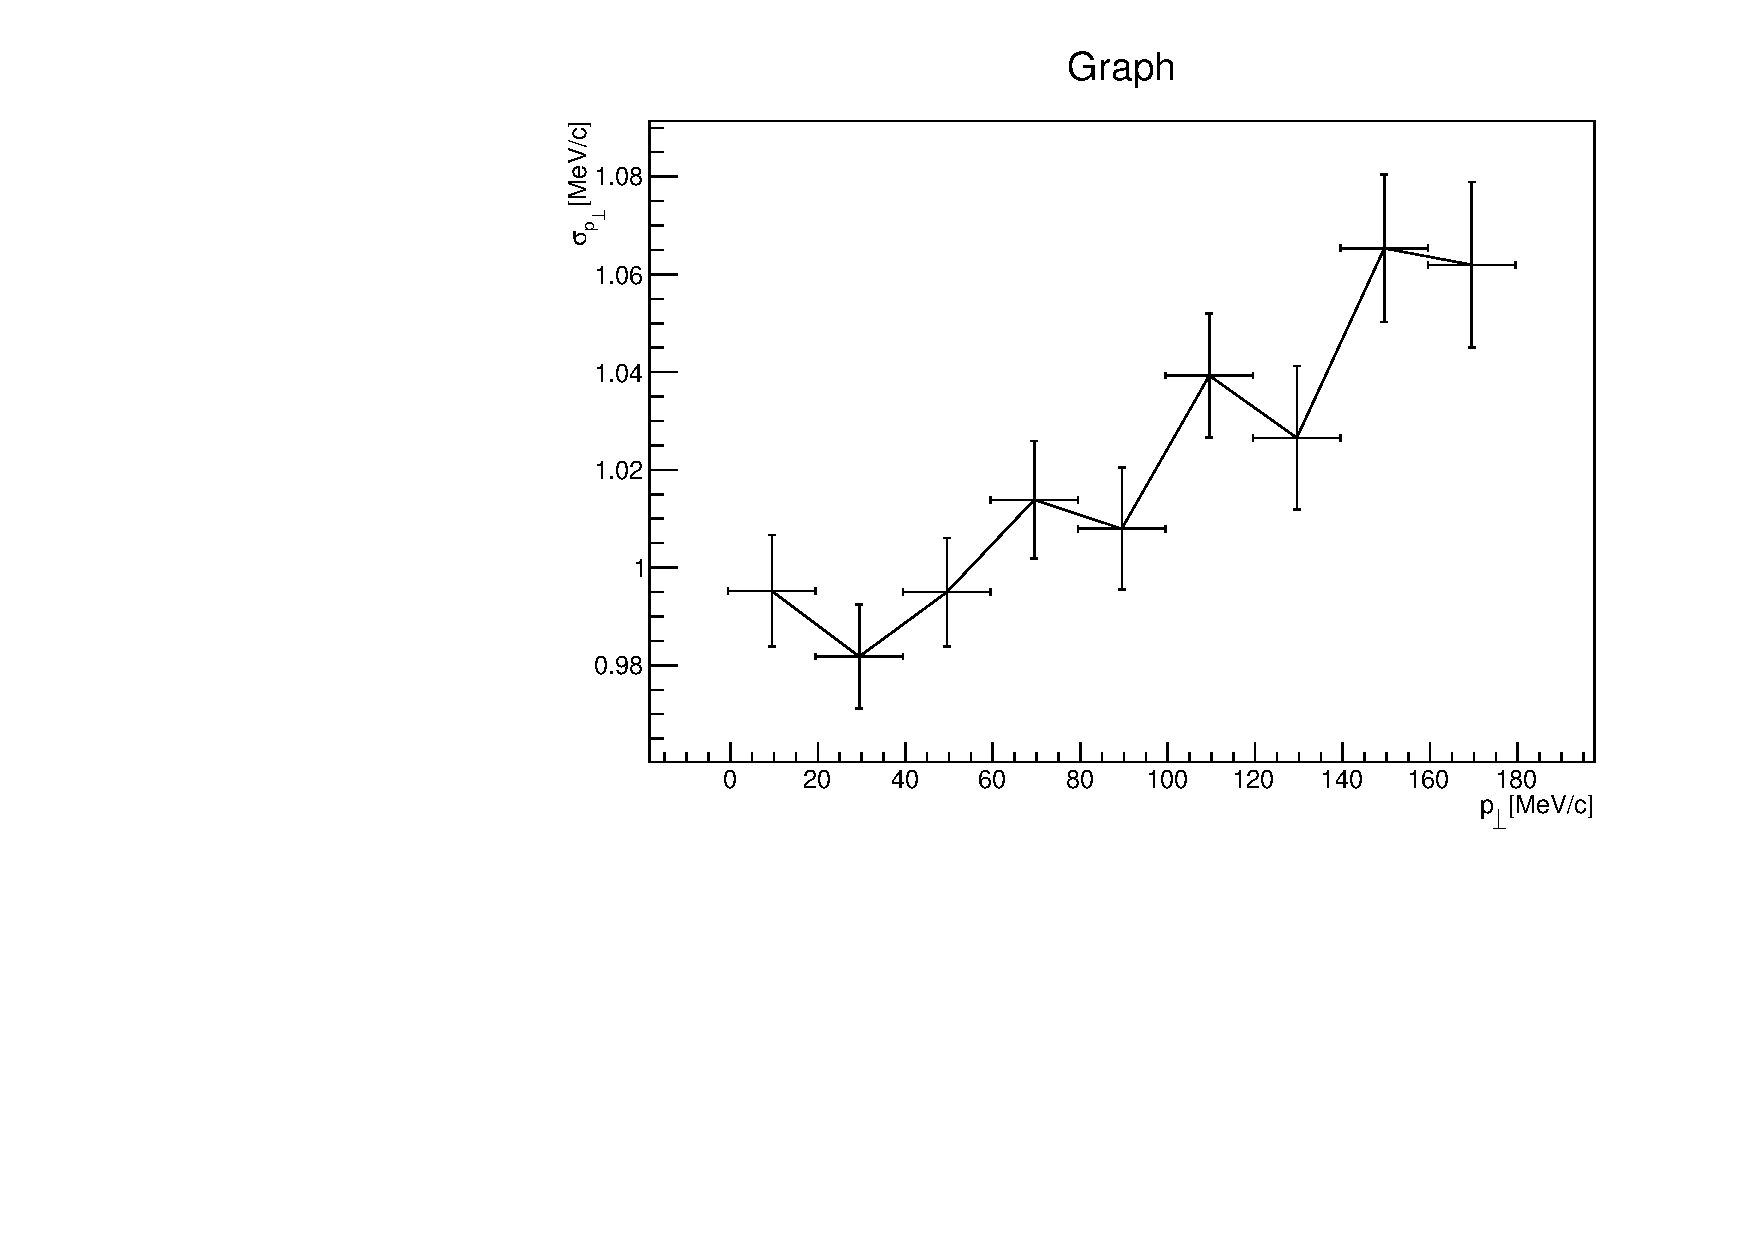
\includegraphics[width=0.49\textwidth, angle=0]{08-Performance/upstream_pt_resolution_vs_pt.pdf}
     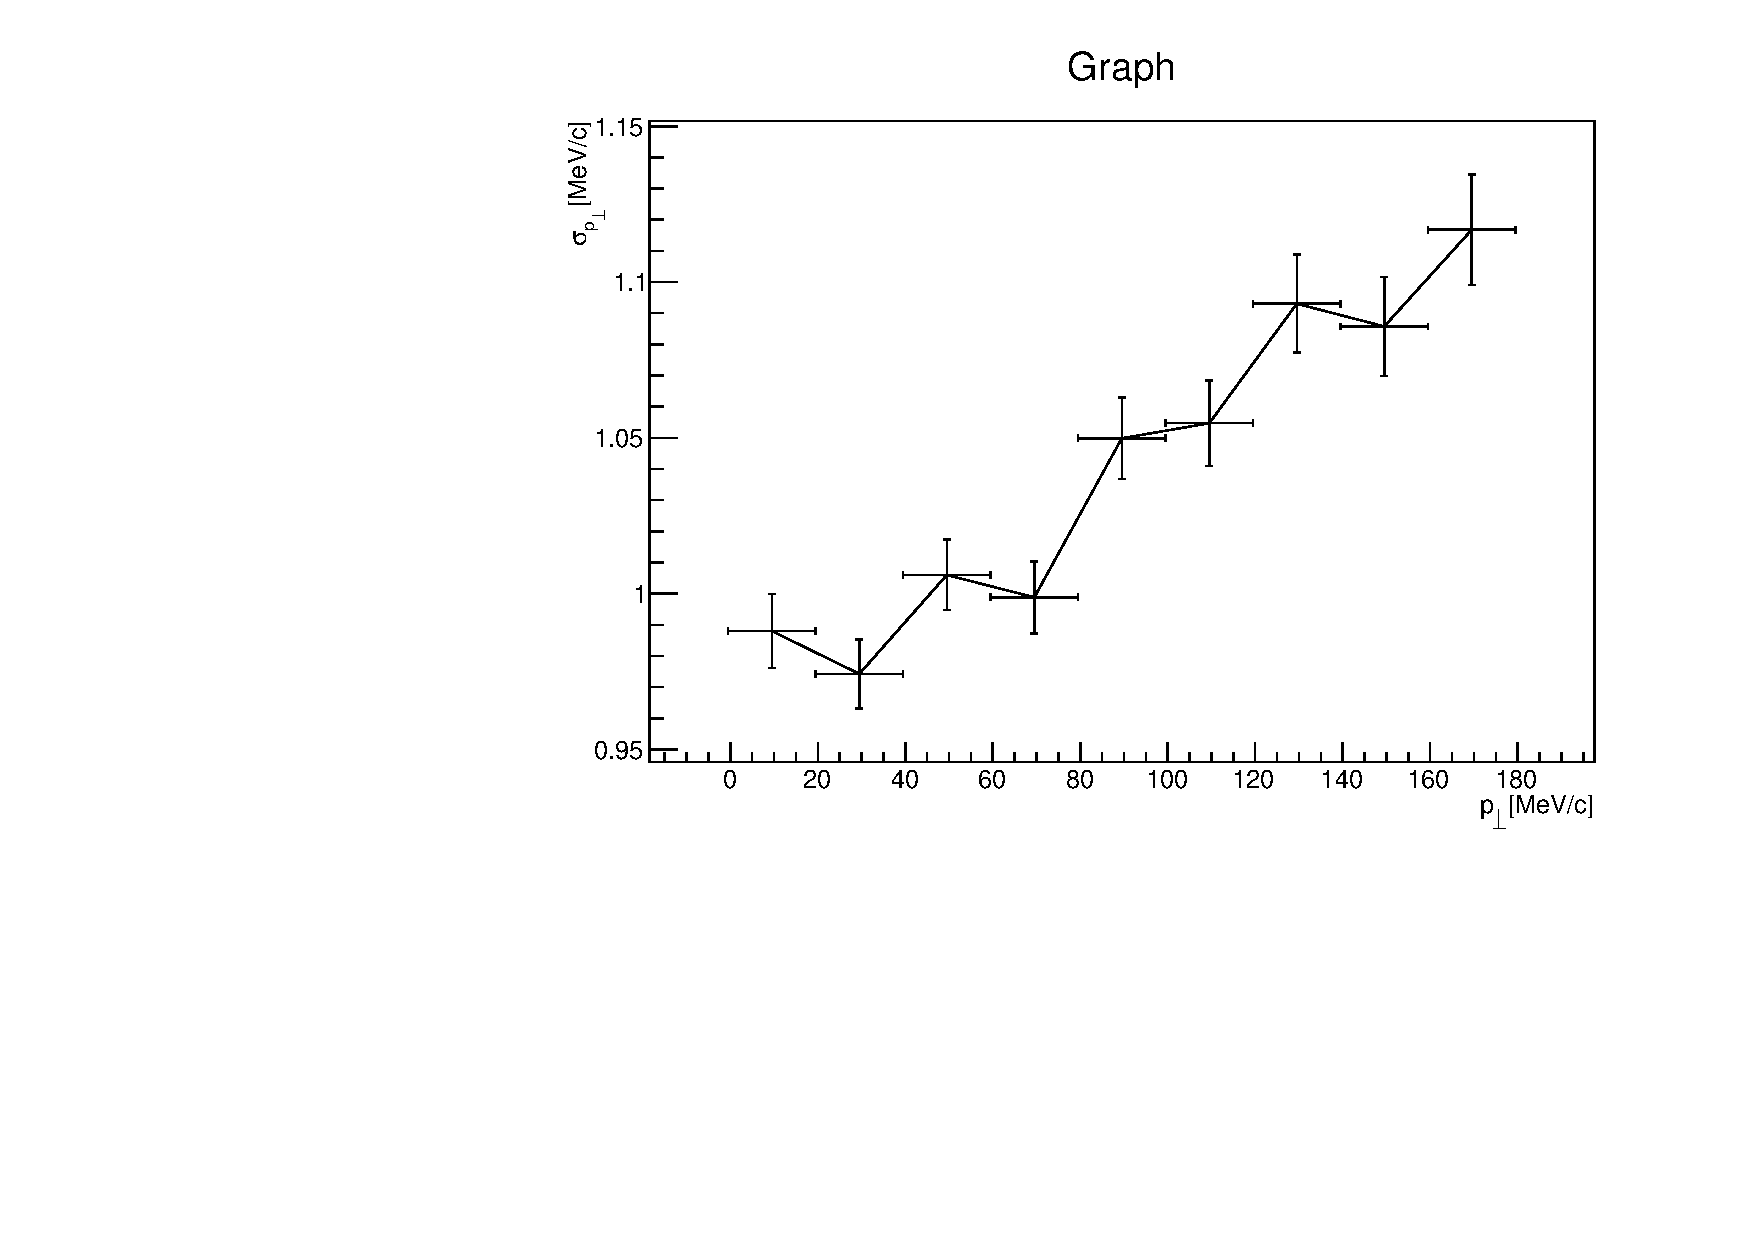
\includegraphics[width=0.49\textwidth, angle=0]{08-Performance/downstream_pt_resolution_vs_pt.pdf}
     \caption{\label{fig:PtPtResolKalman} The $p_t$ resolution vs the $p_t$ of the upstream (left) and downstream (right).}
   \end{center}
  \end{figure}
  
  \begin{figure}[p]
   \begin{center}
     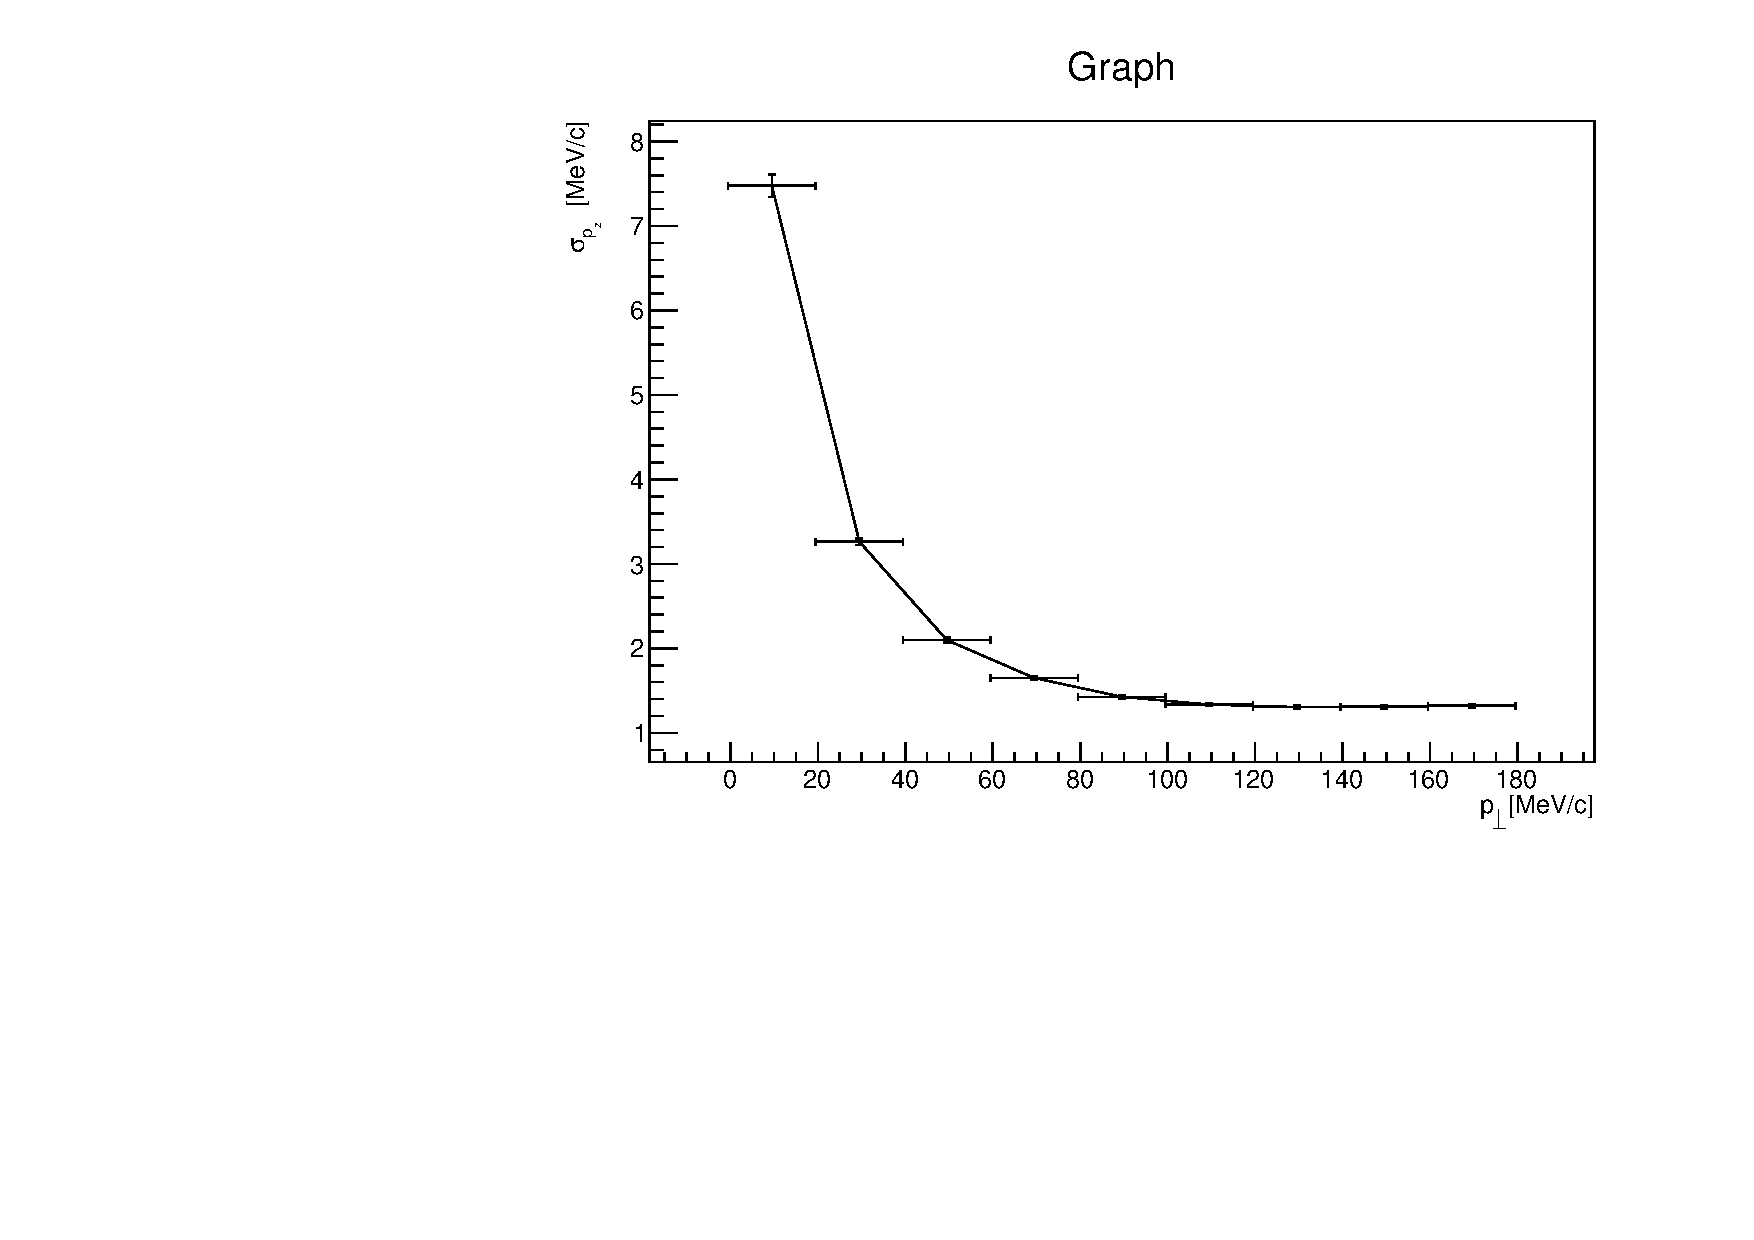
\includegraphics[width=0.49\textwidth, angle=0]{08-Performance/upstream_pz_resolution_vs_pt.pdf}
     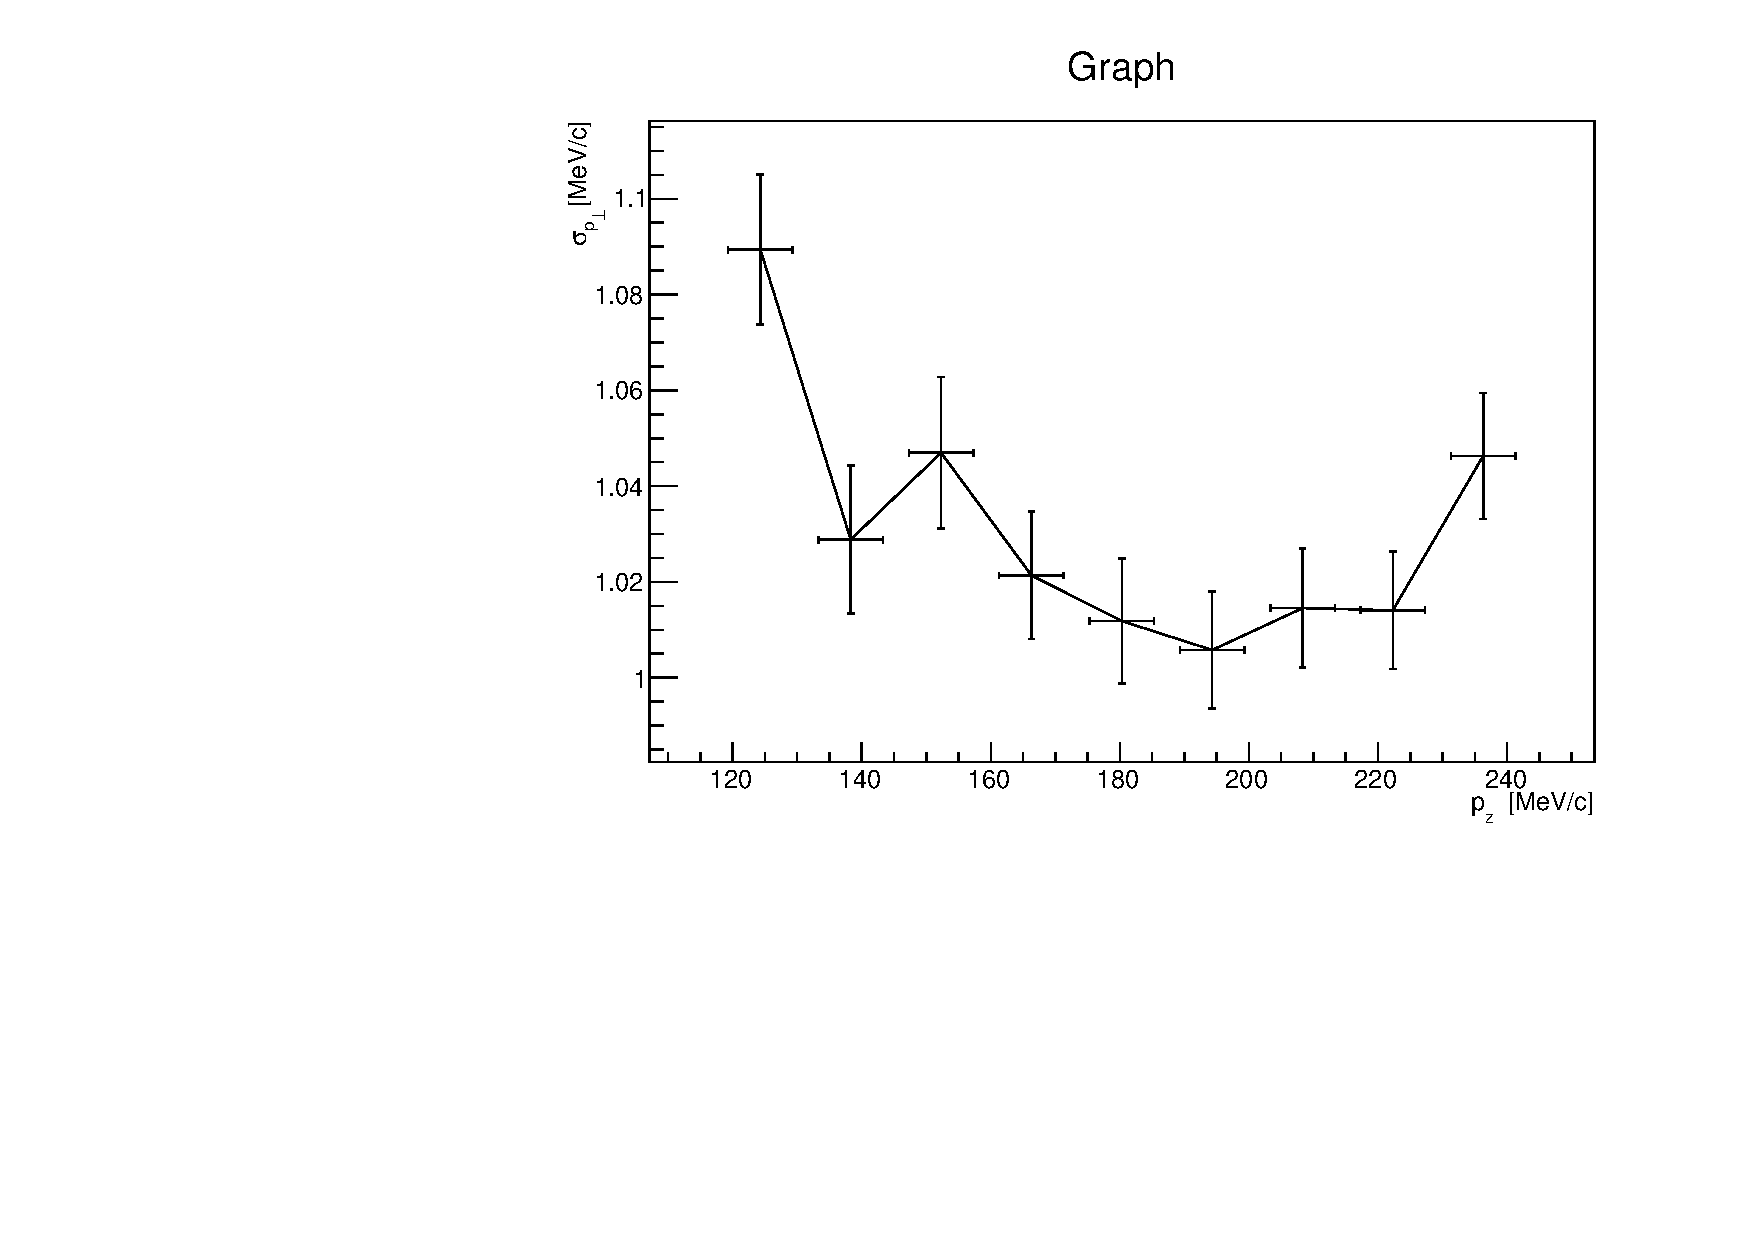
\includegraphics[width=0.49\textwidth, angle=0]{08-Performance/downstream_pz_resolution_vs_pt.pdf}
     \caption{\label{fig:PtPzResolKalman} The $p_z$ resolution vs the $p_t$ of the upstream (left) and downstream (right).}
   \end{center}
  \end{figure}
